\chapter{Qubit calibration}

In this chapter I will describe the process of calibration for superconducting flux-tunable transmon on the hardware located in the QRC (Quantum Research Center) Laboratory of the TII (Technology \& Innovation Institute) in Abu Dhabi.

\section{Experimental setup}
Most of the results presented in this work were obtained using the Contralto-D chip \cite{qw11q}, which offers up to 21 fully connected qubits and 4 isolated qubits, for a total of 25 physical qubits.
The distinction between fully connected and isolated qubits is important as only the fully connected subset supports native two-qubit gate operations, which are essential for implementing entangling gates and complex quantum circuits. 
Isolated qubits, while still operational for single-qubit tasks, do not participate in multi-qubit interactions and thus are not functionally equivalent in terms of computational capabilities.
The topology of the qubit is shown in Figure \ref{fig:qw11q_topology}.

\begin{figure}[ht!]
    \centering
    \begin{subfigure}{0.40\textwidth}
        \centering
        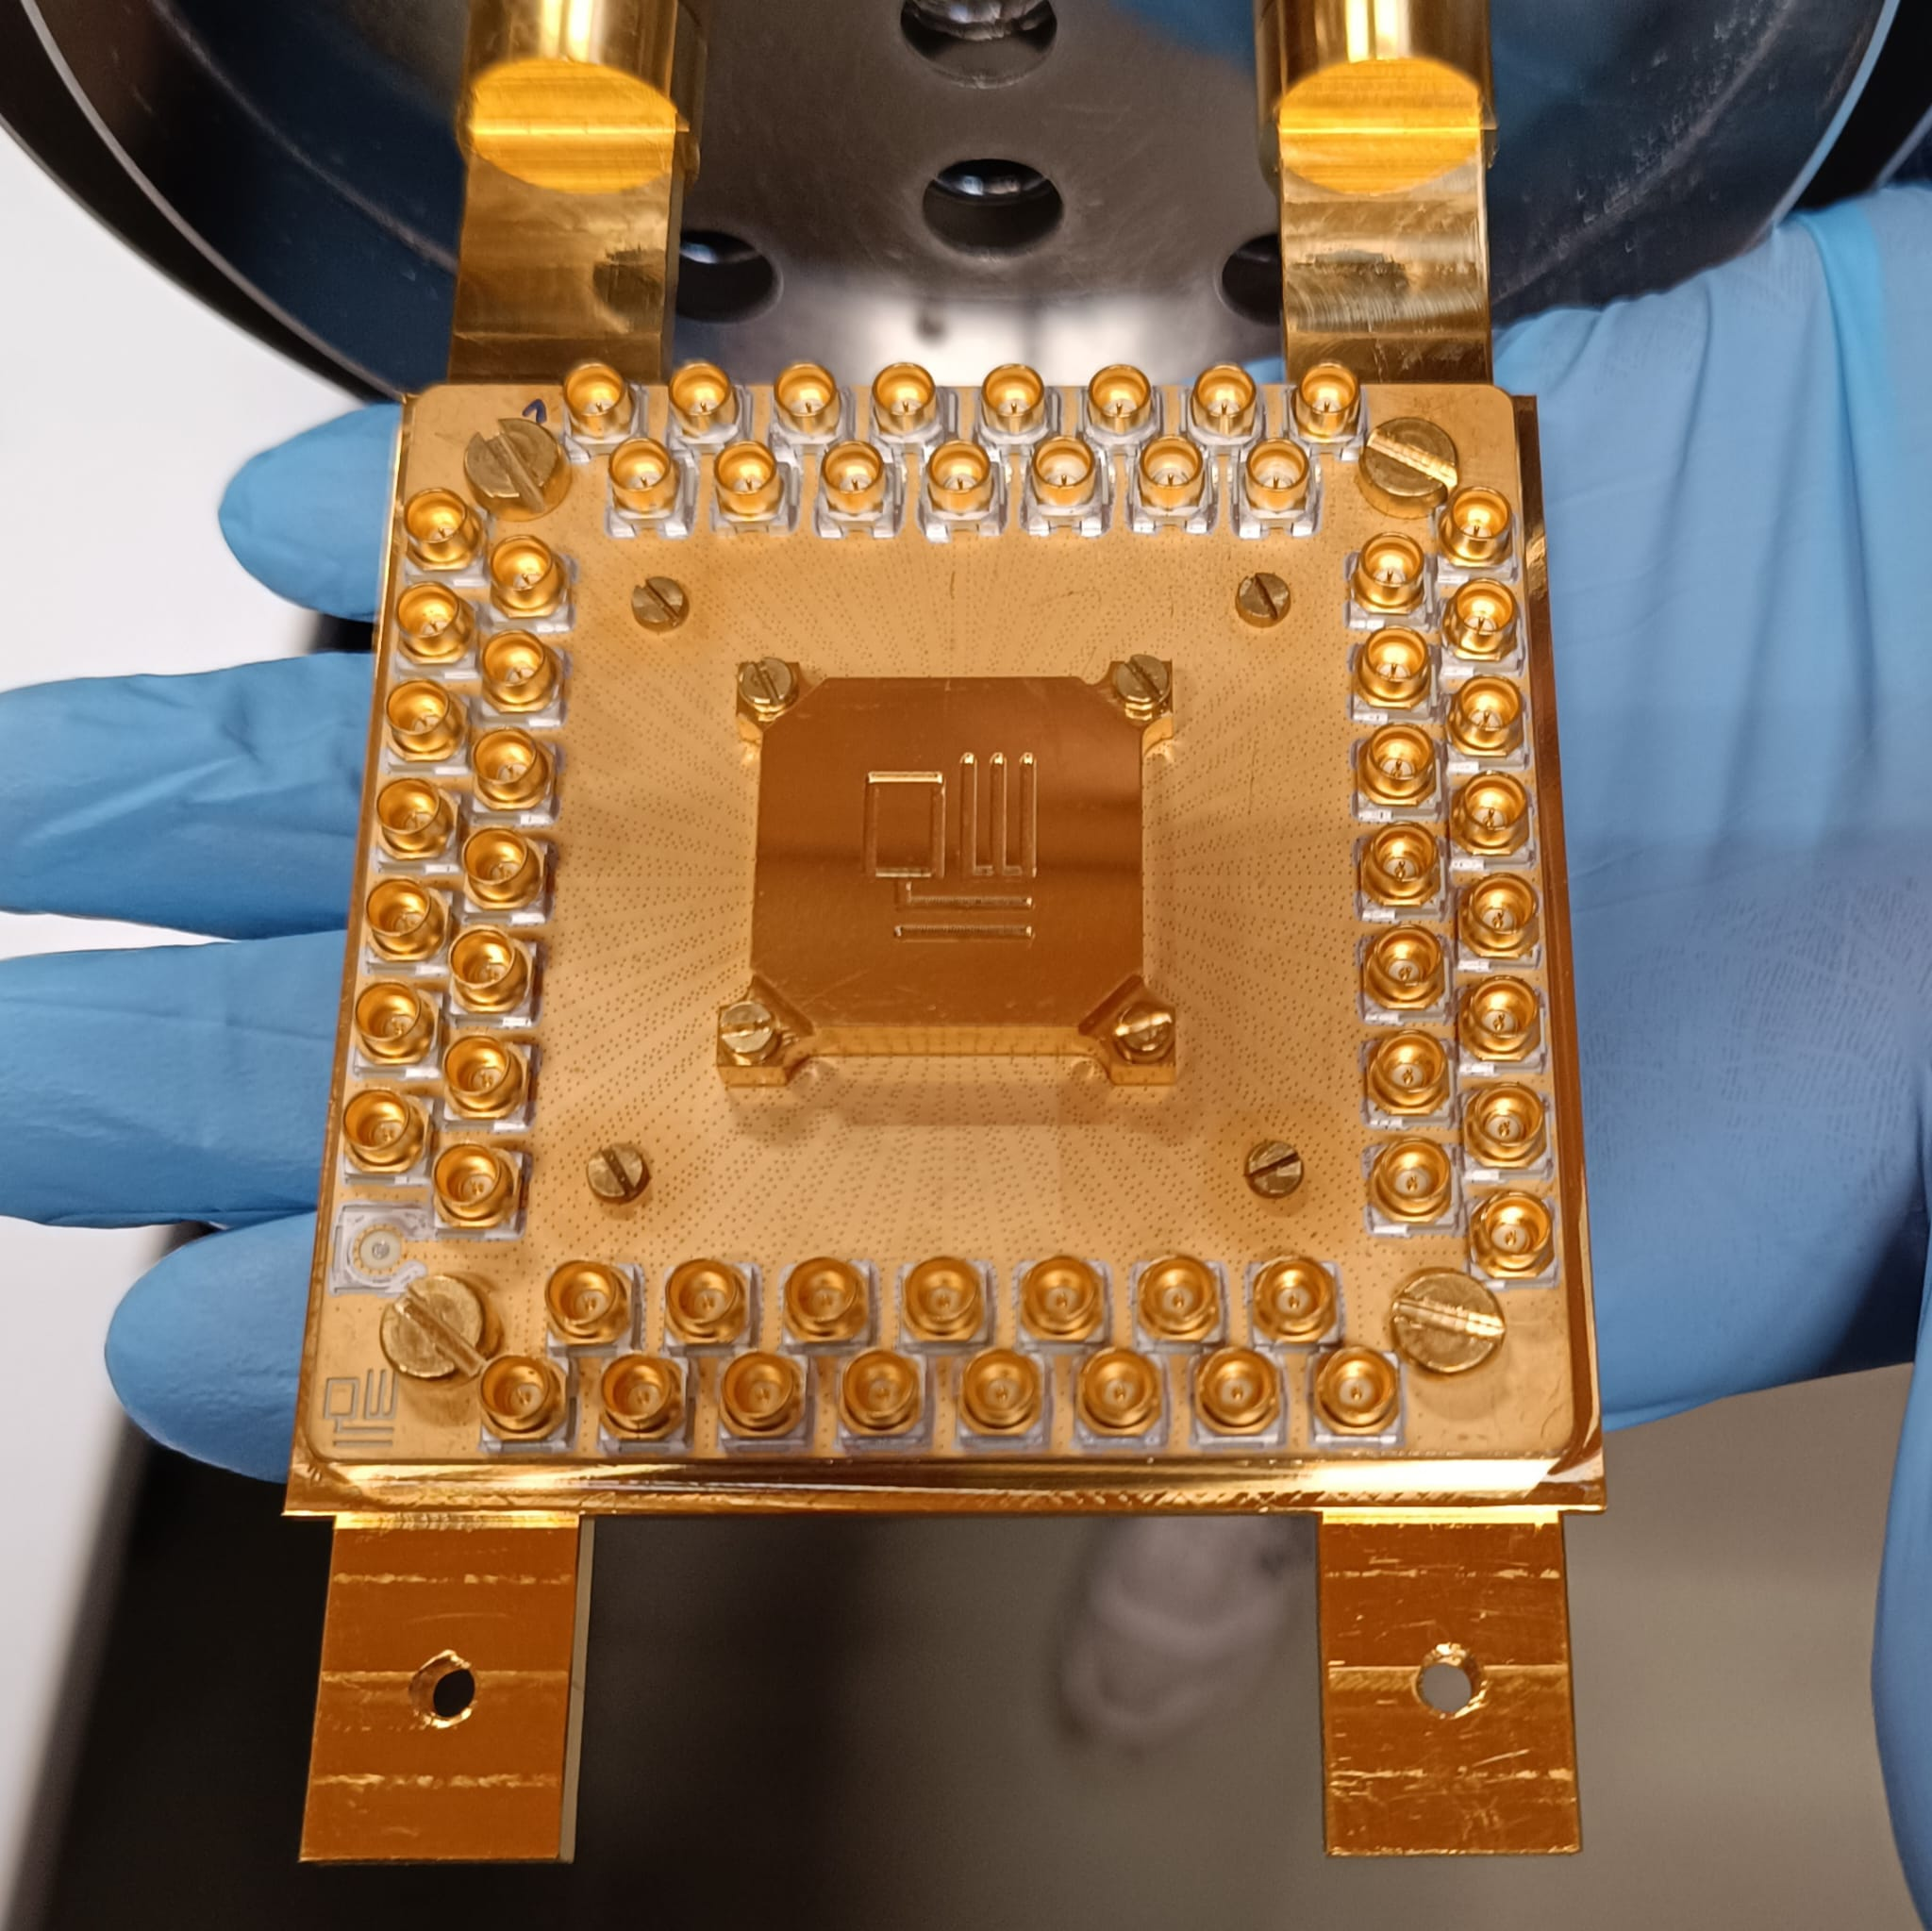
\includegraphics[width=0.80\textwidth]{figures/png/qw11q.jpeg}
        \subcaption{}
        \label{fig:qw11q_picture}
    \end{subfigure}
    \hfill
    \begin{subfigure}{0.50\textwidth}
        \centering
        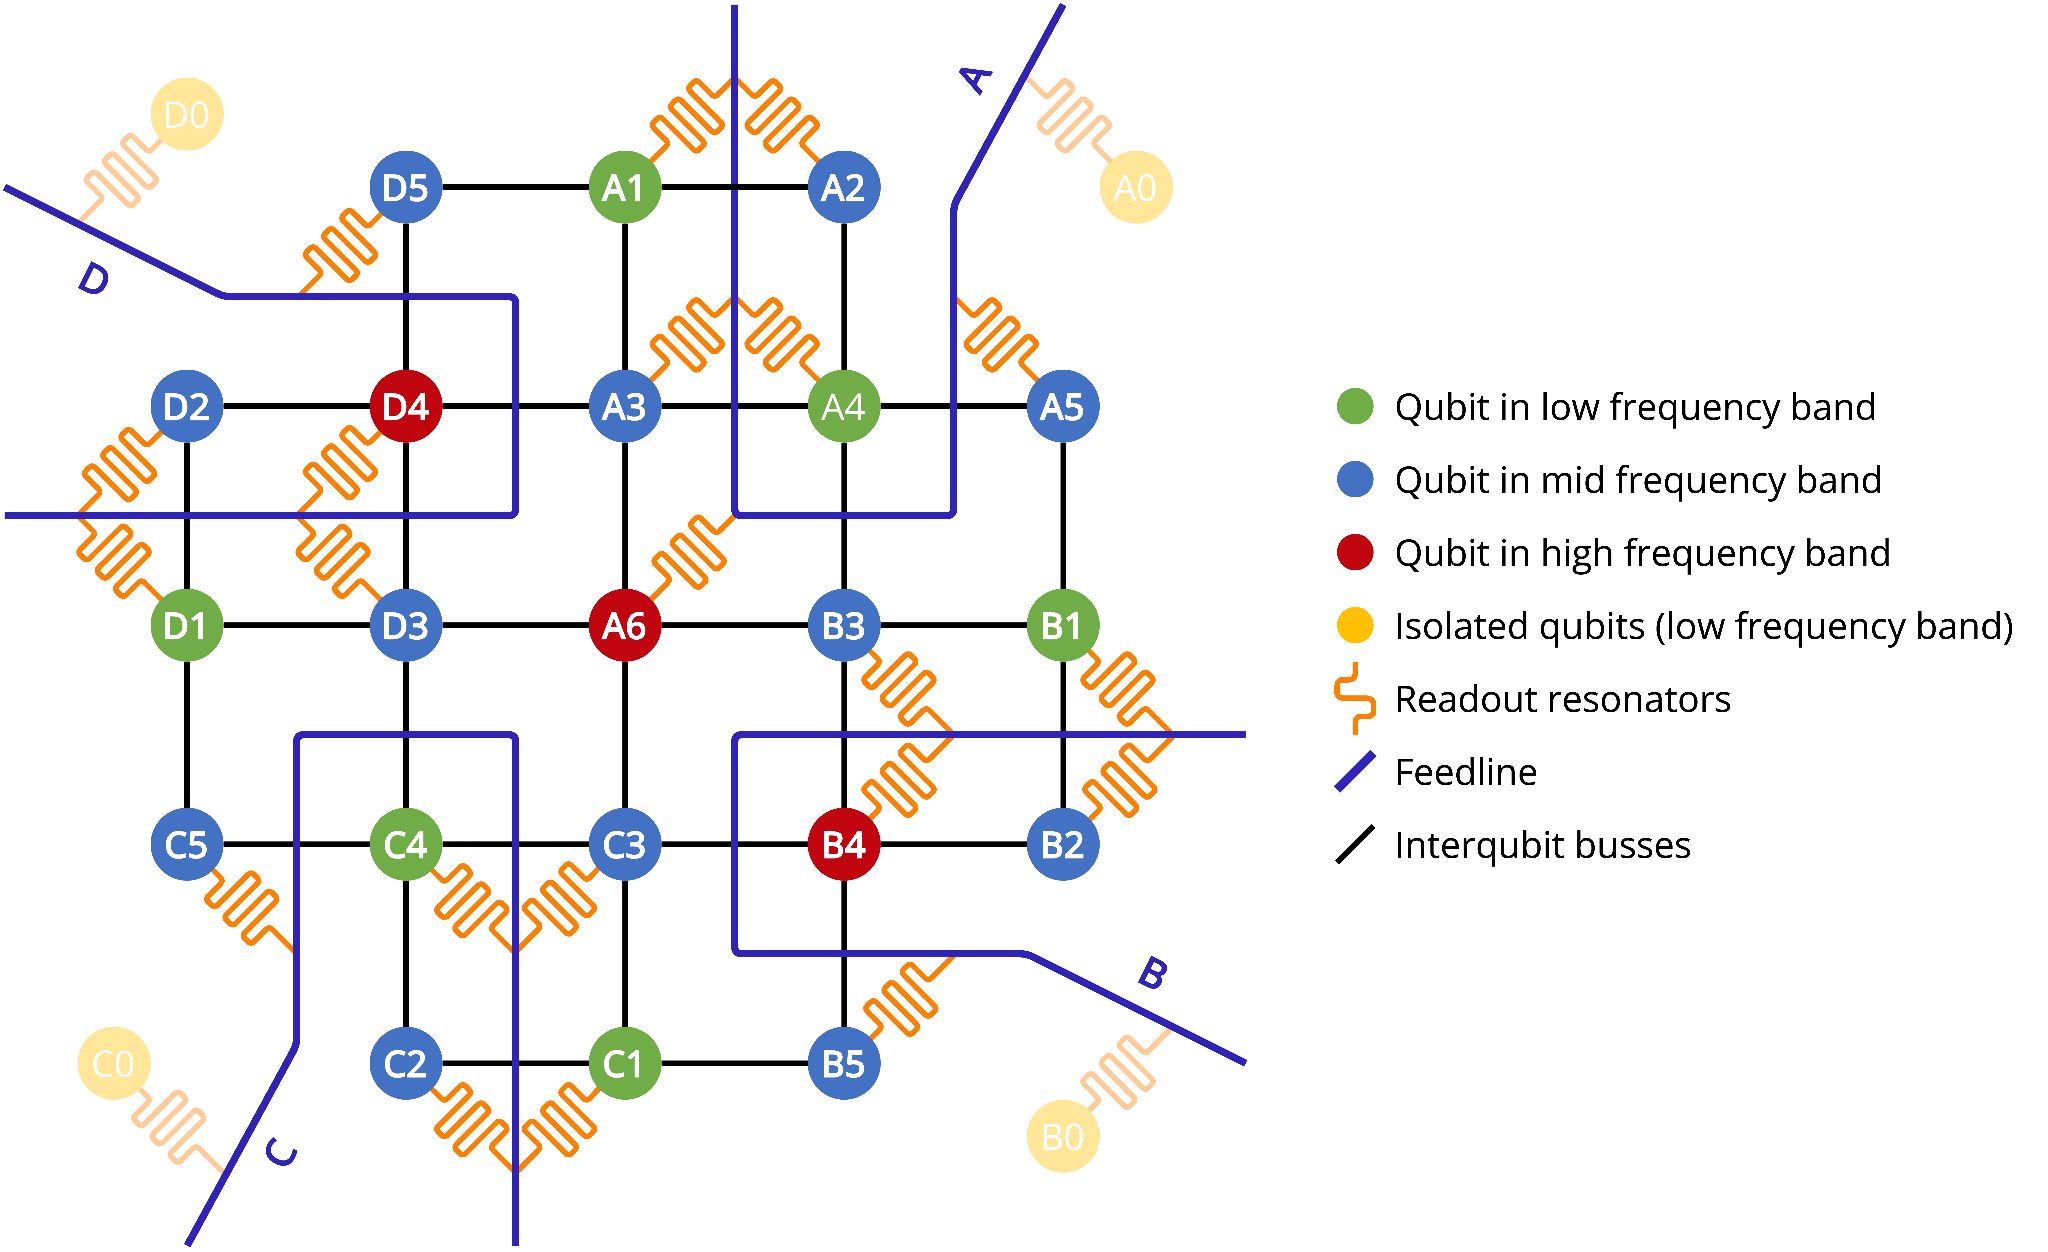
\includegraphics[width=\textwidth]{figures/png/qw11q.png}
        \subcaption{}
        \label{fig:qw11q_topology}
    \end{subfigure}
    \caption{Figure \ref{fig:qw11q_picture}: Picture of the Contralto-D chip from QuantWare. Figure \ref{fig:qw11q_topology}: Topology of the Contralto-D chip from QuantWare.}
    \label{fig:qw11q}
\end{figure}

As discussed in the previous chapter, the behavior of Josephson junctions and SQUIDs relies critically on the superconducting state of the materials involved. 
To achieve and maintain this regime, it is essential that the superconducting elements operate well below their critical temperature. 
For this reason, the Contralto-D chip is installed at the lowest temperature stage of the cryostat, where the required thermal conditions for superconductivity are met. 
This ensures the proper functioning of the quantum hardware and enables the realization of coherent quantum operations.

These systems achieve ultra-low temperatures by exploiting the unique quantum properties of helium-3 (\ce{^{3}He}) and helium-4 (\ce{^{4}He}) isotopes in a dilution process.
At the core of a dilution refrigerator is a mixing chamber, where the cooling mechanism takes place. 
When a mixture of \ce{^{3}He} and \ce{^{4}He} is cooled below approximately 870 millikelvin, the two isotopes phase-separate into a \ce{^{3}He}-rich phase and a \ce{^{3}He}-dilute phase. 
The key principle is that when \ce{^{3}He} atoms cross the phase boundary—from the concentrated phase into the dilute phase—they absorb energy from their surroundings. 
This process is endothermic and is the fundamental source of cooling in the dilution refrigerator.\\
The system operates as a closed loop: \ce{^{3}He} gas is circulated using a combination of sorption pumps and still pumps, which remove \ce{^{3}He} vapor from the still (typically at $600–800$ mK), recondense it at a higher stage, and reintroduce it into the mixing chamber. 
The refrigerator includes several thermalization stages—typically at $50$ K, $4$ K, $800$ mK, $100$ mK, and finally below $20$ mK—each connected to a corresponding cooling stage and separated by radiation shields and thermal filters to minimize heat load and noise from higher-temperature stages.
Dilution refrigerators are highly stable and capable of reaching base temperatures below $10$ mK, with hold times on the order of days or even weeks. 
These temperatures are crucial for achieving the low thermal noise and long coherence times necessary for high-fidelity quantum operations in superconducting circuits.
Specifically, the cryostat employed in the lab is the XLD from Bluefors \cite{XLD1000}, an image of the cryostat is shown in Figure \ref{fig:XLDsl}.

\begin{figure}[h!]
    \centering
    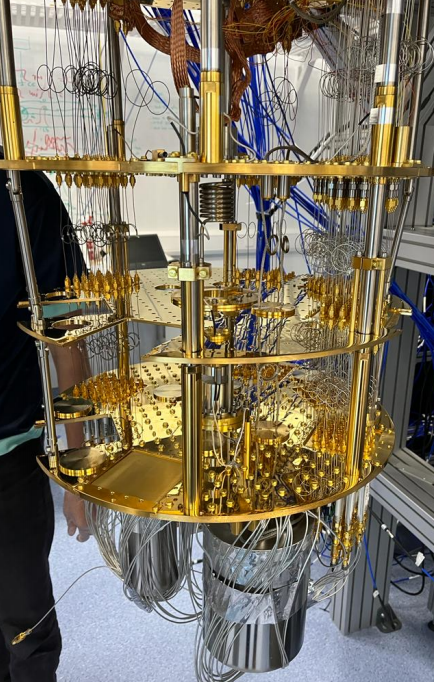
\includegraphics[width=0.35\textwidth]{figures/png/XLD1000.png}
    \caption{Picture of the XLD dilution refrigerator at the QRC Lab}
    \label{fig:XLDsl}
\end{figure}

Outside the cryostat, the control and readout of superconducting qubits are managed by dedicated room-temperature electronics.
These systems are responsible for generating the microwave pulses used to drive single- and two-qubit gates, as well as for acquiring and processing the output signals that encode the qubit states 
Typically they include arbitrary waveform generators (AWGs), microwave sources, mixers, digitizers, and field-programmable gate arrays (FPGAs).
The generated microwave pulses are shaped and modulated at room temperature before being attenuated and routed to the cryogenic environment. 
Similarly, signals returning from the qubits are amplified and digitized for state discrimination and further processing. 
The electronics employed in the lab for the control of the \tt{qw11q} is the OPX1000 platform by Quantum Machines \cite{opx1000}.

The software I used for the calibration of the qubits and the subsequent experiments is \Qibocal (\cite{pasquale_qibocal_2024}, \cite{qibocalscience}, \cite{qibocalgit}), while the backend for communication with the laboratory instruments is \Qibolab (\cite{efthymiou_qibolab_2024}, \cite{qibolabscience}, \cite{qibolabgit}).
\Qibolab is the control layer responsible for managing and executing low-level instructions on the hardware, bridging high-level quantum models and physical quantum platforms.
It is designed to support diverse experimental setups and allows the researcher to define custom hardware configurations through a platform abstraction and to execute custom pulse sequences using both commercial and open-source firmware.
The communication between \Qibolab and the quantum hardware is structured and modular, relying on a stack that includes instrument drivers, pulse control logic, and a compiler that translates abstract quantum gates into hardware-specific instructions.
This structure enables compatibility with heterogeneous platforms and facilitates the development of experimental drivers tailored to different laboratory environments.
\Qibocal interfaces directly with \Qibolab to apply calibration protocols on the physical device. The routine deployment takes place through the interpretation of declarative runcards written in YAML.
\Qibocal allows easy execution of pulse sequences, collection of measurement data, and interpretation of the results through the reports that are automatically generated upon completion of the routine.

\section{Single qubit calibration experiments}\label{sec:calibration}

The first task that I needed to complete at the beginning of my thesis work was the calibration of at least a line of the superconducting qubits of the Contralto-D chip using the \Qibocal library.
From this point onward, for the sake of brevity, I will refer to the chip interchangeably as Contralto-D or \tt{qw11q}, which is the name of the node under which it is registered on the QRC computing cluster.
In the following, I will describe the experiments that I performed and comment on the results.

\subsection{Resonator calibration}
Before starting with the calibration of the gates necessary for quantum computing it is necessary to characterize the qubit and calibrate the readout pulses. 
For this reason, the calibration process starts with the characterization of the resonator coupled to the qubit that will be used to perform non-destructive measurements of the qubit state.

\subsubsection{Resonator spectroscopy}
The first step to calibrate the readout pulse is to characterize the resonator is to find the resonator frequency, that is the transition frequency for the resonator. 
At this frequency, a distinct difference in the transmitted signal can be observed depending on the type of resonator used. 
In the case of a 3D cavity resonator, the signal appears amplified, whereas for a 2D planar resonator, the signal tends to be more strongly absorbed. 
Regardless of the resonator type, the response typically exhibits an approximately Lorentzian-shaped peak: this peak is positive for 3D cavities and negative for 2D resonators.

The outcome of this experiment is strongly influenced by the amplitude of the excitation pulse. 
To reliably determine the resonator frequency, the pulse duration can be fixed on the order of microseconds, which is sufficient to observe the relevant signal response.
However, selecting an appropriate amplitude requires more careful consideration. When the amplitude is high, the signal becomes more prominent, improving the signal-to-noise ratio (SNR) and making it easier to identify the resonator's response.
If the amplitude is increased too much, however, it can drive the system out of the superconducting regime.  
In this case, the resonator becomes effectively decoupled from the qubit, and the frequency observed corresponds to the so-called bare resonator frequency.
During the first calibration operations, it is not necessary to have the qubit coupled to the resonator but is helpful to improve the SNR to have a more defined peak in the signal, for this reason, the first calibration routines are run in a high-power regime.

In this experiment the main variables on which the experimenter can operate are the frequency range that is willing to scan and the step of the scan. 
Regarding the frequency range a very wide scan can be useful if nothing is known about the studied resonator, but usually the design parameters are provided by the manufacturer; t is possible that they are not exact, but can give an idea of the region to scan.
Regarding the step for the scan, usually a step of 200 MHz can be used to probe the resonator frequency but can be reduced if a more precise scan is needed. 
An example of measurement of the bare resonator frequency is shown in Figure \ref{fig:res_high}.
 
\begin{figure}[h!]
    \centering
    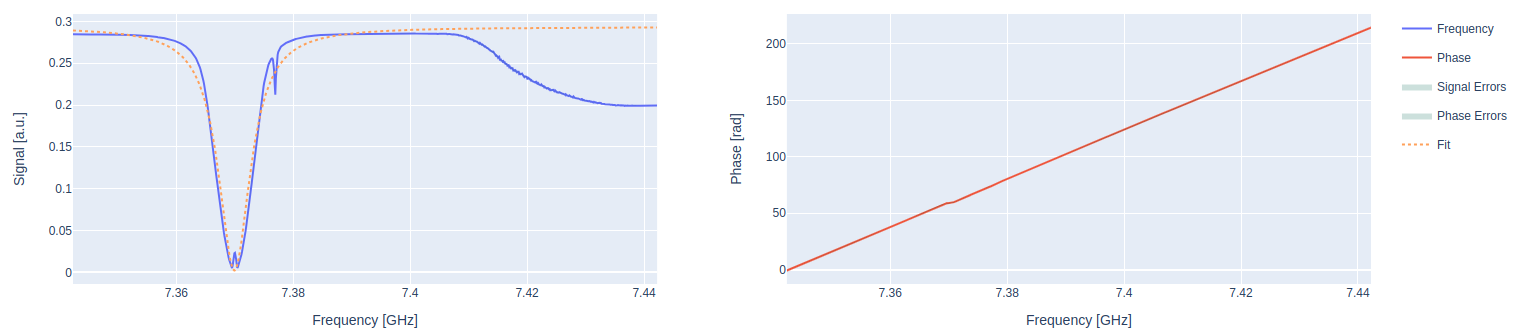
\includegraphics[width=\textwidth]{figures/png/res_spectroscopy_high.png}
    \caption{Output of resonator spectroscopy with high power on qubit B2.}
    \label{fig:res_high}
\end{figure}

An example of the measurement of the resonator frequency in the low-power regime is shown in Figure \ref{fig:res_low}.

\begin{figure}[h!]
    \centering
    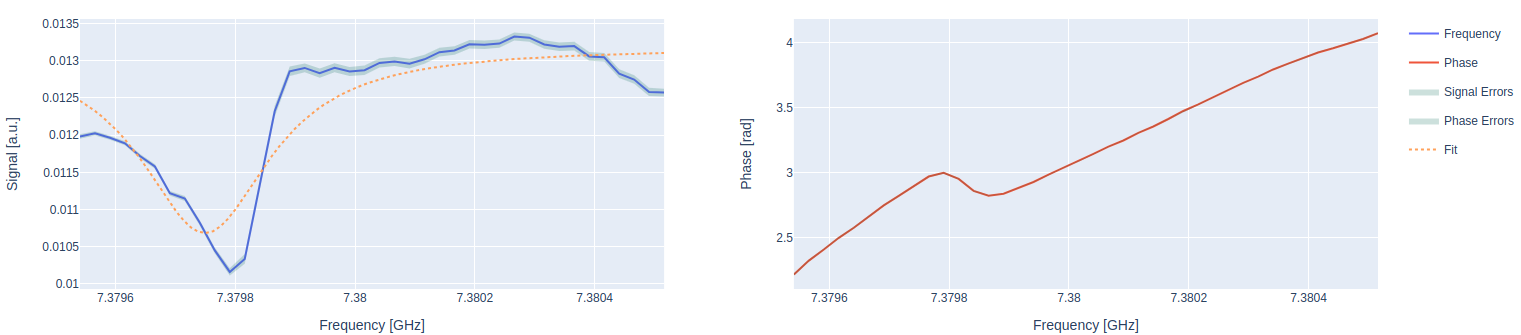
\includegraphics[width=\textwidth]{figures/png/res_low.png}
    \caption{Output of resonator spectroscopy with low power on qubit B2.}
    \label{fig:res_low}
\end{figure}

A more precise study of the resonator's response can be carried out by performing the resonator spectroscopy routine using a different fitting function, the one referred to as \tt{s21} in \Qibocal. 
This variation of the experiment is described in Appendix [\hyperref[app:AppendixA]{Appendix A}].

\subsubsection{Resonator punchout}
After having found the bare resonator frequency it is necessary to identify the the frequency of the resonator when coupled to the qubit. 
To do this it is possible to repeat the spectroscopy, this time over a narrower frequency range and for varying pulse amplitudes. 
The resonator frequency is expected to depend strongly on amplitude: it remains constant in the high-power regime, shifts during an intermediate transition phase, and stabilizes again at a different value once the qubit-resonator interaction becomes significant.
For this calibration protocol, the experimenter must carefully choose the frequency and amplitude range to scan to avoid extremely long experiments, at the same time the frequency and amplitude steps must be small enough to clearly identify the frequency and amplitude in which the shift happens.   

The expected result from a resonator punchout experiment is shown in Figure \ref{fig:res_punchout}
\begin{figure}[h!]
    \centering
    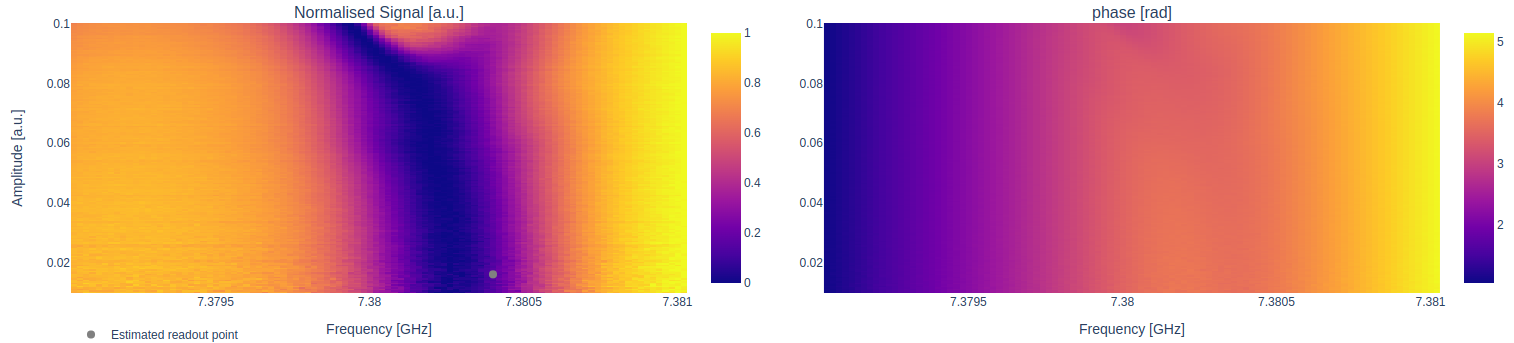
\includegraphics[width=\textwidth]{figures/png/res_punchout.png}
    \caption{Output of resonator punchout on qubit B2.}
    \label{fig:res_punchout}
\end{figure}

\subsubsection{Resonator flux dependence}
As explained in section \ref{subsec:flux_tunable_transmon} it is suggested to work at the qubit sweetspot, where the qubit frequency is less sensitive to magnetic flux fluctuations.
For this reason, it is useful to estimate the location of the sweetspot prior to performing qubit spectroscopy, enabling measurements to be carried out near the optimal bias point. 
This can be accomplished by exploiting the qubit-resonator coupling: since the qubit frequency depends on the magnetic flux, as shown in equation \ref{eq:freqdepndenceonflux}, and the qubit is coupled to the resonator, the resonator frequency also exhibits a flux dependence. 
The resonator detuning in the transmon regime ($E_J \gg E_C$) can be computed as 
\begin{equation}\label{eq:resonator_flux_dependence}
    f_r(\Phi) = f_r^{\text{bare}} + \frac{g^2 \sqrt[4]{d^2 + (1 - d^2) \cos^2 \left( \pi \frac{\Phi}{\Phi_0} \right)}}{f_r^{\text{bare}} - f_q(\Phi)},
\end{equation}
where $f_r^{\text{bare}}$ is the bare resonator frequency, $g$ is the coupling between the transmon and the resonator, $d$ is the junctions asymmetry, $E_C$ is the charging energy, $E_J$ the Josephson energy and $\Phi_0 = h/2e$ is the flux quanta.

In \Qibocal it is possible to perform a resonator flux dependence experiment to measure and fit the curve described by Eq. \ref{eq:resonator_flux_dependence}.
With this routine the experimenter performs a scan of both the external bias and frequency, this experiment provides an approximate indication of the sweetspot.
An example of the output of this experiment is shown in Figure \ref{fig:res_flux_dep}

\begin{figure}[h!]
    \centering
    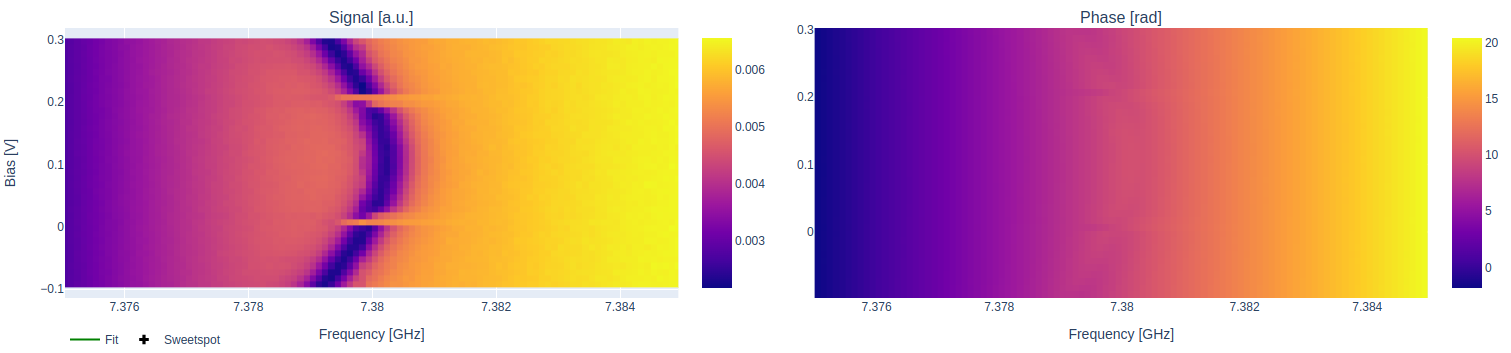
\includegraphics[width=\textwidth]{figures/png/cute_flux.png}
    \caption{Output of resonator flux dependence routine on qubit B2.}
    \label{fig:res_flux_dep}
\end{figure}

\subsection{Qubit calibration}
After having determined all the readout parameters it is possible to continue the calibration process by calibrating the qubit.

\subsubsection{Qubit spectroscopy}
To determine the resonance frequency of a qubit, a qubit spectroscopy experiment is performed, which, unlike resonator spectroscopy, requires a two-tone approach. 
While resonator spectroscopy is typically a single-tone measurement used to identify the resonator's response, qubit spectroscopy involves applying a drive tone to the qubit followed by a readout tone to detect the qubit state. 
This method becomes essential after an initial estimate of the readout frequency and amplitude has been obtained from a resonator punchout experiment. 
In this protocol, a drive pulse of variable frequency $\omega$ is sent through the qubit drive line. 
If the drive frequency is far detuned from the qubit transition frequency $\omega_{q}$, it will have no appreciable effect on the qubit state, and the measured signal will remain unchanged. 
However, as $\omega$ approaches $\omega_{01}$ the drive pulse can induce transitions between the qubit states. 
This excitation modifies the qubit population and, consequently, the resonator response, which is sensitive to the qubit state due to their dispersive coupling. 
When the drive frequency is near resonance and the pulse is sufficiently long, the qubit may reach a maximally mixed state leading to a detectable change in the readout signal amplitude. 
By sweeping the drive frequency and recording the corresponding readout amplitudes, one can plot a spectroscopy curve that reveals a Lorentzian dip or peak centered at the qubit transition frequency—opposite in direction to the Lorentzian feature observed in the resonator spectroscopy, due to the nature of the state-dependent dispersive shift.

An example of the output of a qubit spectroscopy experiment is shown in Figure \ref{fig:qubit_spectroscopy}
\begin{figure}[h!]
    \centering
    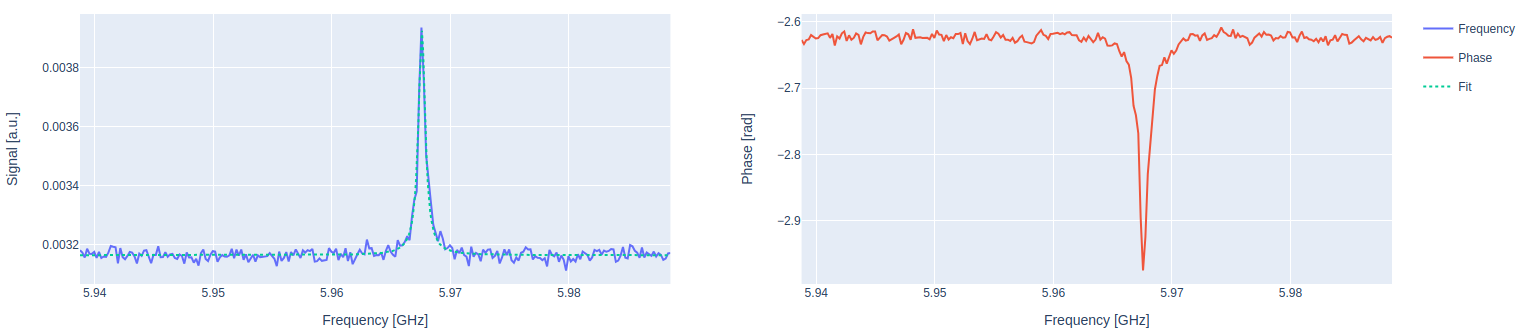
\includegraphics[width=\textwidth]{figures/png/qubit_spectroscopy.png}
    \caption{Output of qubit spectroscopy on qubit B2.}
    \label{fig:qubit_spectroscopy}
\end{figure}

\subsubsection{Qubit spectroscopy for second excited state}
Qubit spectroscopy can also be extended to probe transitions to higher excited states beyond the first excited state. 
Directly observing these higher-level transitions typically requires significantly increased drive power, which may exceed the safe operational limits of the experimental setup. 
An alternative and more controlled approach involves first preparing the qubit in state $\ket{1}$, followed by a standard spectroscopy sequence to induce the $\ket{1} \leftrightarrow \bra{2}$ transition. 

%\begin{figure}[h!]
%    \centering
%    \includegraphics[width=\textwidth]{figures/png/ef.png}
%    \caption{Output of qubit spectroscopy to identify the transition frequency between state $\ket{1}$ ($\ket{e}$) and state $\ket{f}$ (first scited state) on qubit B2.}
%    \label{fig:ef}
%\end{figure}

Note that the description of this calibration routine has been included here for the sake of clarity and continuity of exposition; however, since it requires the qubit to be in the $\ket{1}$ state at the beginning of the spectroscopy, it can only be performed after the execution of a single-shot classification (see Section \ref{subsec:single_shot}).

\subsubsection{Qubit flux dependence}
By performing a resonator flux dependence the experimenter obtained a first estimate for the sweetspot, which can be improved by performing a qubit flux spectroscopy.
In this experiment, a constant DC current signal is sent to the qubit through the flux line with voltage and amplitude fixed for the bias level and then a qubit spectroscopy is performed.
This procedure is repeated for different bias levels and different drive frequencies.
The expected result of the routine is shown in Figure \ref{fig:qubit_flux}.

When calibrating the qubit sweetspot it is important to consider that on a superconducting quantum chip qubits are not completely isolated systems; rather, they interact with one another through both intentional couplings (e.g capacitive or inductive couplers) and unintended cross-talk mechanisms. 
The mutual interaction between qubits affects their effective operating parameters, particularly their flux-dependent transition frequencies.
This means that also the location of the sweetspot can be affected by the biasing of neighboring qubits, this occurs because the flux-tuning circuitry is not perfectly isolated; biasing one qubit can induce a spurious flux in nearby qubits, effectively shifting their frequency spectra and hence their sweetspots.
Consequently, calibrating each qubit in isolation may yield misleading results, therefore, to accurately determine and operate all qubits at their true sweetspots under realistic experimental conditions, it is important to perform simultaneous calibration. 
This ensures that all mutual interactions and cross-couplings are properly accounted for, leading to a more stable and predictable multi-qubit operation.

\begin{figure}[h!]
    \centering
    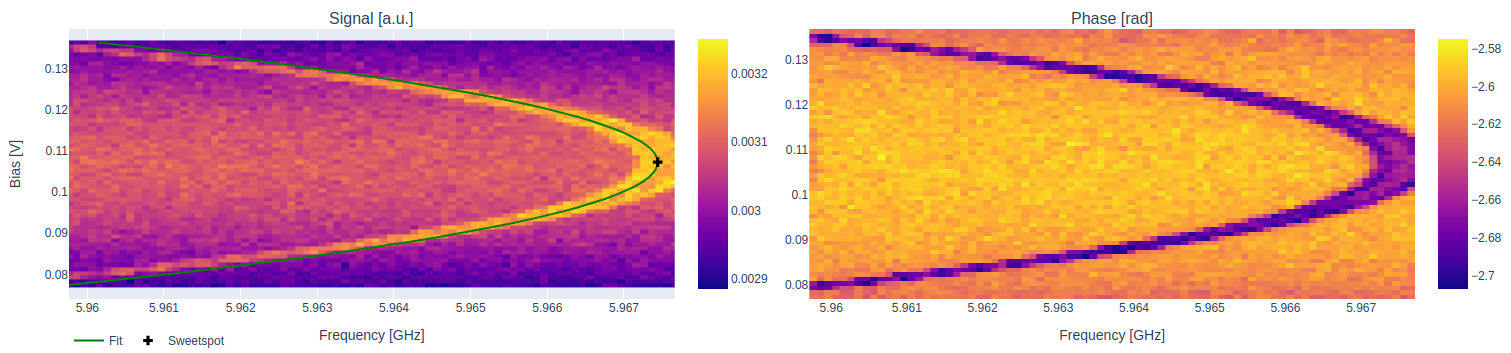
\includegraphics[width=\textwidth]{figures/png/qubit_flux.png}
    \caption{Output of the qubit flux dependence on qubit B2.}
    \label{fig:qubit_flux}
\end{figure}

\subsection{Drive pulse calibration}\label{sec:Rabi}

After defining all the readout parameters and the parameters for qubit control, it is necessary to calibrate the parameters of the drive pulses to be able to control rotations on the Bloch sphere.
With Rabi experiments are possible to calibrate the drive pulses to perform precise rotations (see \cite{Rabi1936}, \cite{Wallraff2005}) within approximately $40$ ns.
This duration is typical for single-qubit gates in superconducting qubit systems, as it represents a balance between fast control and minimal spectral leakage. 
Faster gates would require higher drive amplitudes, which can increase errors due to leakage into higher transmon levels or induce unwanted transitions in nearby qubits through cross-resonance or crosstalk effects \cite{TransmonPaper}, \cite{Motzoi_2009}. 
On the other hand, significantly longer gates are more susceptible to decoherence, particularly due to $T_1$ relaxation and $T_2$ dephasing processes, which limit overall gate fidelity \cite{Barends2014-pb}.

Usually, the first step of calibrating drive pulses consists of calibrating a $\pi$-pulse, namely an $X$-gate. 
The goal of the Rabi experiment is to tune the amplitude or duration of the drive pulse, to excite the qubit from the ground state up to state $\ket{1}$.

\subsubsection{Rabi oscillation experiments}
To experimentally probe the coherent control of a qubit in \Qibocal it is possible to perform different variations of the Rabi oscillation experiments, which provides direct evidence of the qubit's ability to undergo controlled rotations under a resonant microwave drive, as described in Section \ref{sec:qubit_control}.
In this experiment, a microwave pulse of the form  

\begin{equation}\label{eq:microwave_pulse}
    V_d(t) = A \varepsilon(t) \sin(\omega_d t + \alpha),
\end{equation}
is applied through the control line (XY line), and coupled capacitively to the qubit. 
The qubit is initialized in its ground state $\ket{0}$, and the drive frequency $\omega_d$ is set close to the qubit transition frequency $\omega_q$. 
The envelope $\varepsilon(t)$ is typically Gaussian, and its shape is kept constant throughout the experiment. 
The key parameter that is varied is the amplitude $A$ of the drive pulse (or alternatively, the duration of the pulse while keeping amplitude constant).

To better understand the evolution of the system, it is possible to consider the driven qubit in the interaction picture. 
The qubit state can be written as:
\begin{equation}\label{eq:general_state}
    \ket{\psi(t)} = C_0(t) e^{+i \omega_q t/2} \ket{0} + C_1(t) e^{-i \omega_q t/2} \ket{1}.
\end{equation}
%
Solving the time-dependent Schr\"odinger equation for state \ref{eq:general_state} under Hamiltonian\ref{eq:interaction_hamiltonian} yields the following expressions:
\begin{align}
    C_0(t) &= e^{-i \Delta_d t / 2} \left[ \cos \left( \frac{\Omega_R t}{2} \right) + i \frac{\Delta_d}{\Omega_R} \sin \left( \frac{\Omega_R t}{2} \right) \right], \\
    C_1(t) &= i \frac{\Omega}{\Omega_R} e^{i \Delta_d t / 2} \sin \left( \frac{\Omega_R t}{2} \right),
\end{align}
where $\Delta_d = \omega_q - \omega_d$ is the detuning, and
\begin{equation}
    \Omega_R = \sqrt{\Omega^2 + \Delta_d^2},
\end{equation}
is the generalized Rabi frequency.

The probability of finding the qubit in the excited state at time $t$ is given by:
\begin{equation}\label{eq:P1_rabi}
    P_1(t) = |C_1(t)|^2 = \frac{\Omega^2}{\Omega^2 + \Delta_d^2} \sin^2 \left( \frac{\Omega_R t}{2} \right).
\end{equation}
This result shows that the probability oscillates in time with frequency $\Omega_R$, and the amplitude of the oscillation is reduced when the drive is off-resonant ($\Delta_d \neq 0$).
The closer the drive is to resonance, the higher the probability of full excitation.

In the resonant case, when $\omega_d =\omega_q$ and $\Delta_d = 0$ the generalized Rabi frequency reduces to $\Omega_R = \Omega$ and the excited state probability becomes
\begin{equation}\label{eq:rabi_amplitude}
    P_e (t) = P_1(t) = \sin^2\left(\frac{\Omega t}{2} \right) = \frac{1}{2}(1-\cos(\Omega t)),
\end{equation}
which is the curve that is used in the fit when performing a Rabi amplitude experiment.

An example of the output of a Rabi amplitude experiment is shown in figure \ref{fig:rabi_amplitude}.
\begin{figure}[h!]
    \centering
    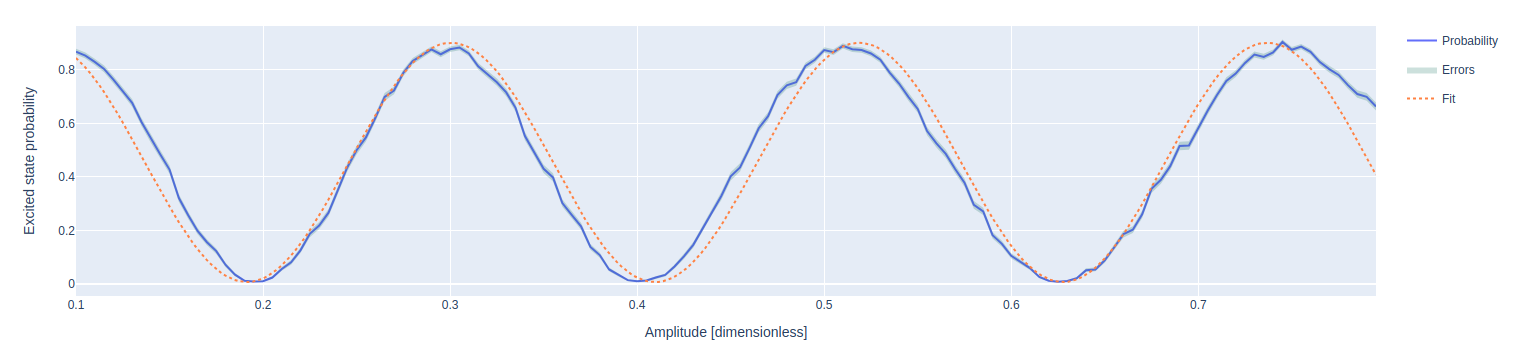
\includegraphics[width=\textwidth]{figures/png/rabi_amp.png}
    \caption{Output of the Rabi amplitude routine on qubit B2.}
    \label{fig:rabi_amplitude}
\end{figure}

A variation of the Rabi amplitude experiment consists of the Rabi length experiment, where instead of the amplitude, the parameter that is varied is the duration of the drive pulse.
The qubit is again initialized in the ground state $\ket{0}$ and subjected to a resonant microwave drive ($\omega_d = \omega_q$). 
In this case, the pulse envelope $\varepsilon(t)$ and amplitude $A$ are held constant, while the total duration of the pulse is incrementally varied. 
This enables the observation of coherent oscillations in the excited state population as a function of pulse length. 
However, unlike the idealized scenario, in realistic conditions, the qubit experiences energy relaxation and dephasing, which attenuate the oscillation amplitude over time. 
To account for these effects, the excited state probability is modeled as represents the effective decay time, incorporating both energy relaxation and dephasing processes.
\begin{equation}
    P_e (t) = P_1(t)= \frac{1}{2}\left(1- e^{-t/\tau}\cos(\Omega_R \frac{t}{2})\right),
\end{equation}
where $\Omega_R$ is the generalized Rabi frequency and $\tau$ 

\begin{figure}[h!]
    \centering
    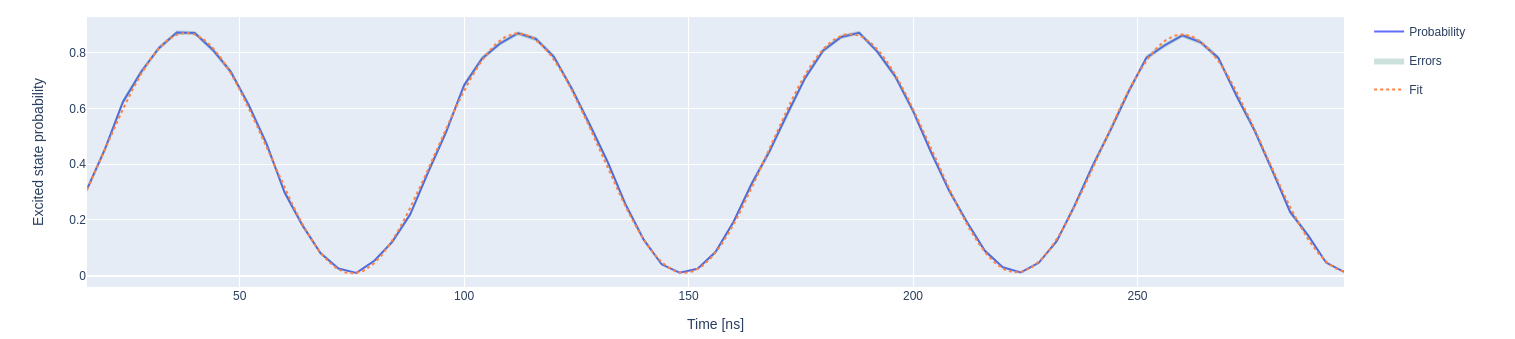
\includegraphics[width=\textwidth]{figures/png/rabi_length.png}
    \caption{Output of the Rabi length routine on qubit B2.}
    \label{fig:rabi_length}
\end{figure}


Sometimes, when the qubit frequency is not precisely known, or when systematic effects such as pulse distortions, frequency drifts, or cross-talk may affect the calibration it can be useful to perform a Rabi measurement in which the amplitude and frequency of the drive pulse are scanned.
In \Qibocal this experiment is implemented as the Rabi amplitude-frequency routine, this experiment provides a comprehensive view of the qubit's response to a range of drive conditions and is particularly useful during initial calibration.
This experiment reveals a characteristic chevron-shaped interference pattern in the excitation probability as a function of drive frequency and amplitude. 
Figure \ref{fig:rabi_amplitude_frequency} shows a possible output of this experiment, in the plot in figure in particular it is possible to see only the first region of the chevron shape with high probability of finding the qubit in an excited state.

\begin{figure}[h!]
    \centering
    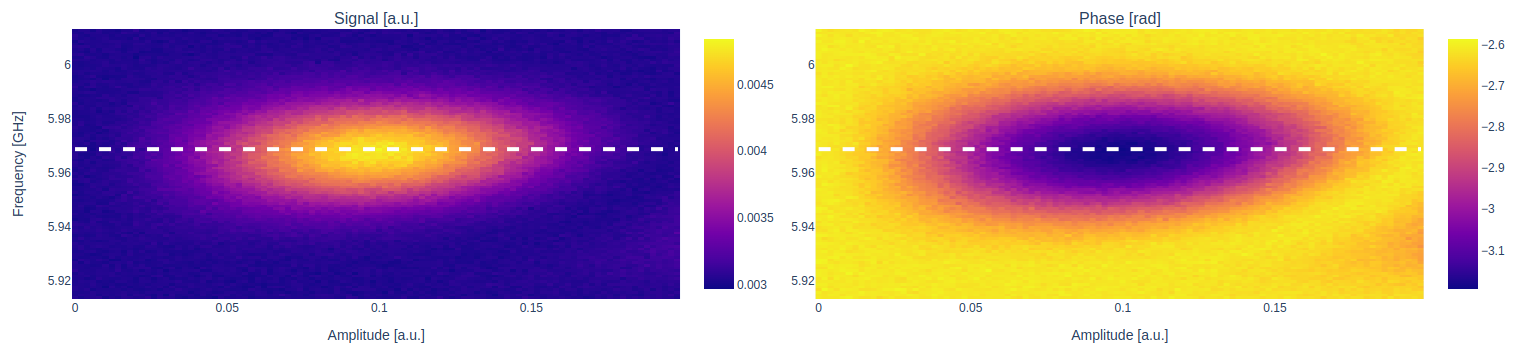
\includegraphics[width=\textwidth]{figures/png/rabi_af.png}
    \caption{Output of the Rabi amplitude-frequency routine on qubit B2.}
    \label{fig:rabi_amplitude_frequency}
\end{figure}

\subsection{Single shot classification}\label{subsec:single_shot}
At this stage of the calibration procedure, the drive and measurement pulses have been individually calibrated, while a measurement now yields a clear analog output, this alone does not indicate whether the qubit was in state $\ket{0}$ or $\ket{1}$.
To establish this correspondence and enable digital state assignment, it is necessary to perform a single-shot readout experiment.

To characterize the readout configuration of a superconducting qubit, the measurement is performed using a heterodyne detection setup (see \cite{gao_practical_2021}, \cite{krantz_quantum_2019}) which acquires the transmitted microwave signal from the readout resonator.
Although the average signal clearly distinguishes the two states, in a single instance, often called a "single shot", the signal is noisy. 
This noise arises both from quantum fluctuations intrinsic to the electromagnetic field inside the resonator and from added noise contributed by amplifiers and other electronics in the detection chain.
The raw signal, sampled over a finite window, is digitally integrated to produce a single complex number corresponding to one measurement instance.
Repeating this process after preparing the qubit in a known state produces a cloud of points in the complex IQ plane \cite{krantz_quantum_2019}.
For both state $\ket{0}$ and state $\ket{1}$ we typically observe one Gaussian-shaped distribution of IQ values The separation between these two clusters originates from the dispersive interaction between the qubit and the resonator, which induces a state-dependent frequency shift and consequently a distinguishable phase shift in the transmitted microwave tone. 
Since the acquisition integrates the signal over time, each shot produces a single point whose location reflects the qubit state but is blurred by the noise that generates the Gaussian distributions.

The readout calibration experiment starts by preparing the qubit in state $\ket{0}$, letting it relax to its ground state, and collecting IQ data without averaging.
The experiment is then repeated after applying a $\pi$-pulse to prepare the qubit in state $\ket{1}$ and the IQ-values are recorded.
Plotting all these single shots in the IQ plane reveals two roughly circular clusters. 

To classify the measured IQ points, the centroids of the two Gaussian-like distributions corresponding to the qubit prepared in $\ket{0}$ and $\ket{1}$ are first identified. 
The axis passing through these centroids is used to define the direction along which the state information is most distinguishable. 
The IQ plane is then rotated so that this axis aligns with the horizontal (real) axis, concentrating the relevant state-dependent variation along a single dimension. 
This rotation is characterized by an angle, measured in radians, between the centroid-connecting axis and the original $Q$-axis.

Following the rotation, the coordinate system is translated such that the centroid of the ground state distribution is placed at the origin. 
All IQ points are then projected onto the real axis, and the resulting one-dimensional distributions for each state are analyzed. 
The cumulative distribution functions of these projections are computed, and the optimal threshold is determined by finding the point that maximizes the absolute difference between the two distributions. 
This threshold defines the decision boundary used to assign a binary qubit state to any new measurement, based on its projection along the rotated axis.

The quality of the classification is then quantified by the assignment fidelity, defined as \cite{gao_practical_2021} 
\begin{equation}
    \mathcal{F} = 1 -\frac{1}{2}(P(0,1)+P(1,0)),
\end{equation}
where $P(i,j)$ is the probability of measuring the qubit in state $i$ but prepared in state $j$; this fidelity is typically expected to exceed 90–95\% for a well-calibrated readout. 
It serves as a crucial figure of merit for the qubit, reflecting how reliably one can distinguish its quantum states in a single-shot measurement. 

The result of the classification routine should be similar to the one shown in Figure \ref{fig:classification}.

\begin{figure}[h!]
    \centering
    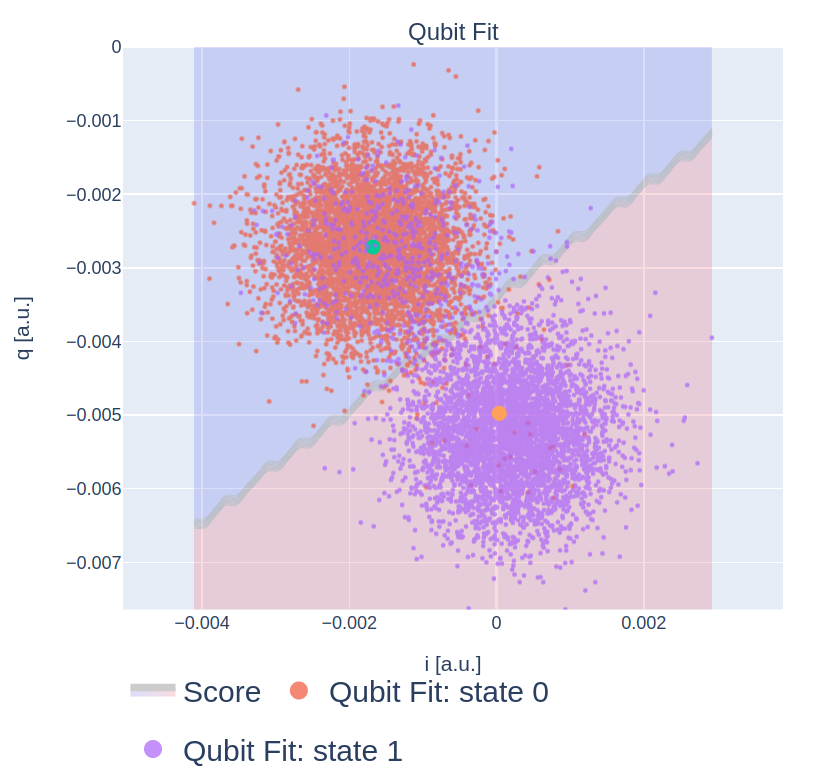
\includegraphics[width=0.4\textwidth]{figures/png/classification.png}
    \caption{Output of the single shot classification on qubit B2.}
    \label{fig:classification}
\end{figure}

\subsection{Fine-tuning calibration}

\subsubsection{Ramsey experiment}\label{subsec:Ramsey}
After calibrating the readout and $\pi$-pulses, technically should be possible to execute algorithmic experiments on the qubit. 
However, essential characteristics of the qubit, such as its coherence properties and the precise drive frequency, remain to be determined; without this information, circuit fidelities would be suboptimal. 
The Ramsey experiment is a simple yet powerful protocol that allows simultaneous investigation of multiple aspects of qubit behavior, including the fine-tuning of the drive frequency and verification of coherent control and signal phase consistency. 
It also enables the extraction of the qubit's coherence time $T_2^*$.

In its standard implementation, the Ramsey sequence consists of two $\frac{\pi}{2}$-pulses separated by a variable delay $\tau$.\\
The first $\frac{\pi}{2}$-pulse brings the qubit from the ground state $\ket{0}$ onto the equatorial plane of the Bloch sphere, placing it in a superposition of $\ket{0}$ and $\ket{1}$.
During the delay $\tau$, he qubit state accumulates a relative phase due to its Larmor precession and environmental noise, effectively evolving around the z-axis.\\
The second $\frac{\pi}{2}$-pulse projects the final state back onto the measurement basis, and the probability of measuring the excited state $\ket{1}$ is recorded.
Repeating this procedure for different delay times $\tau$ allows us to monitor the decay of coherence in the qubit state.

In the ideal, non-detuned case, where the drive frequency matches the qubit transition frequency, the observed signal exhibits a purely exponential decay toward a baseline value, from which the characteristic decoherence time $T_2^*$ can be extracted.
However, small deviations from the ideal $\frac{\pi}{2}$-pulse, due to imperfect calibration or a mismatch between the drive and qubit frequency lead to more complex behavior.

Usually, a small intentional detuning is applied, in this case, the measurement outcomes show a sinusoidal modulation superimposed on the exponential decay so that the resulting curve can be fitted with the equation \cite{Baur2012RealizingQG}
\begin{equation}\label{eq:Ramsey}
    p_e(\tau) = \frac{1}{2} + \frac{1}{2}e^{-\tau/T_2^*}\cos{(\Delta\omega \tau)},
\end{equation}
An example of the output of a Ramsey experiment is shown in Figure \ref{fig:ramsey}

\begin{figure}[h!]
    \centering
    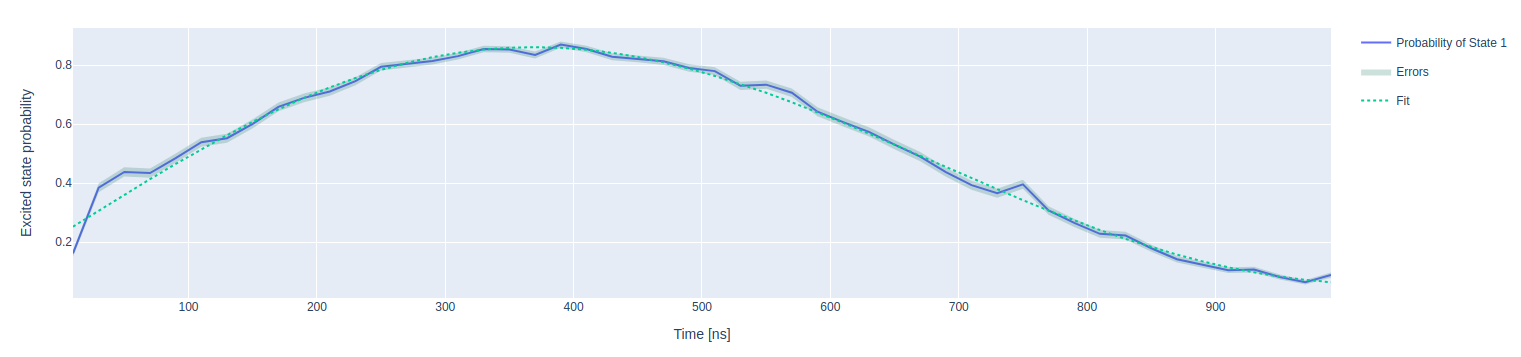
\includegraphics[width=\textwidth]{figures/png/ramsey.png}
    \caption{Output of the Ramsey amplitude routine on qubit B2.}
    \label{fig:ramsey}
\end{figure}

\subsubsection{Flipping experiment}\label{subsec:Flipping}

While the Ramsey experiment is typically used to fine-tune the drive frequency of a qubit, the Flipping experiment serves as an effective routine to calibrate the amplitude of the $\pi$-pulse, ensuring accurate implementation of $R_x(\pi)$ rotations. 
This calibration is fundamental for achieving high-fidelity gate operations, and the flipping experiment can often reveal discrepancies in the amplitude that are not evident in Rabi oscillation measurements.\\
In this protocol, a flip is defined as a pair of consecutive $\pi$-pulses, which ideally return the qubit to its initial state due to a full $2\pi$ rotation. 
The experiment begins with the qubit initialized in the ground state $\ket{0}$, followed by an $R_x(\pi/2)$ rotation that places it in an equal superposition state on the equator of the Bloch sphere. 
Without the initial $R_x(\pi/2)$ rotation, errors in the $\pi$-pulses would lead only to a global phase difference, which is not detectable via projective measurements. 
With the superposition state, however, the qubit's evolution becomes sensitive to amplitude miscalibrations, allowing over- and under-rotations to be distinguished through changes in measurement probability.

Following the initial $\pi/2$-pulse, the qubit is subjected to a number $N$ of flips chosen by the experimenter. 
After the flips, a projective measurement is performed. This procedure is repeated for increasing values of $N$, effectively building a scan of how the qubit state evolves under repeated application of imperfect $\pi$-pulses.

In the ideal case, where the $\pi$-pulse amplitude is perfectly calibrated, the repeated flips return the qubit to the equatorial plane after each cycle, resulting in a constant measurement probability. 
The recorded signal should appear as a flat line; however, if the amplitude is miscalibrated, the qubit state will drift on the Bloch sphere, leading to oscillatory behavior in the measured population as a function of the number of flips. 
This deviation is modeled by a sinusoidal function, from which the amplitude error can be quantitatively extracted.
Figure \ref{fig:flipping} shows the result of a flipping routine.

\begin{figure}[h!]
    \centering
    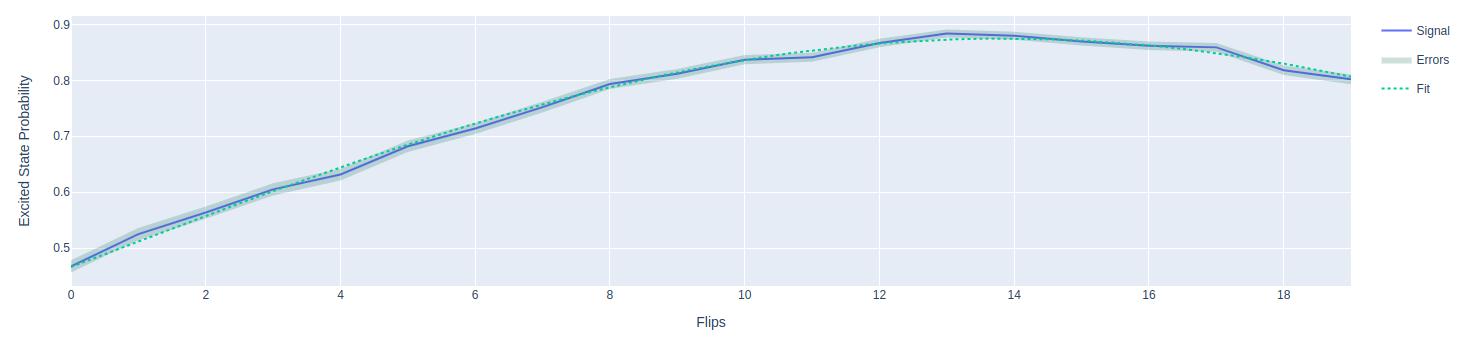
\includegraphics[width=\textwidth]{figures/png/flipping.png}
    \caption{Output of the flipping routine on qubit B2.}
    \label{fig:flipping}
\end{figure}

\subsubsection{Dispersive shift}
A possible strategy to improve the assignment fidelity is to perform a dispersive shift measurement which helps calibrate the readout frequency.
To calibrate the readout frequency based on the dispersive shift, two resonator spectroscopy measurements are performed. 
In the first, the resonator response is measured while the qubit remains in its ground state $\ket{0}$, effectively treating the system as a bare resonator. 
In the second measurement, a calibrated $\pi$-pulse is applied before each acquisition to prepare the qubit in the excited state $\ket{1}$, and the spectroscopy is repeated under otherwise identical conditions. 
The transmission or reflection spectra from both configurations are then plotted together as a function of probe frequency. 
At each frequency point, single-shot measurements are collected, and the resulting IQ data are analyzed. 
Specifically, the distance between the centroids of the two resulting IQ distributions, one corresponding to the ground state and the other to the excited state, is computed. 
The readout frequency that maximizes this centroid separation is selected, as it provides the greatest distinguishability between the two qubit states and thus optimizes the readout contrast.

A typical result for this routine is shown in Figure \ref{fig:dispersive_shift}

\begin{figure}[h!]
    \centering
    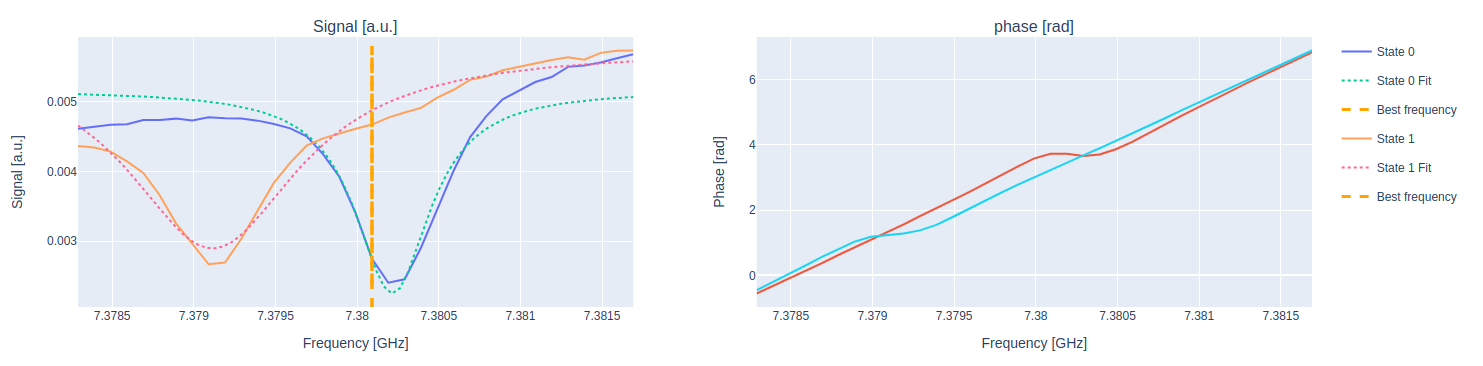
\includegraphics[width=\textwidth]{figures/png/dispersive_shift.png}
    \caption{Output of the Rabi amplitude routine on qubit B2.}
    \label{fig:dispersive_shift}
\end{figure}

\subsection{Qubit characterization}
\subsubsection{T1 \& T2 measurement}
After having calibrated all the parameters concerning the qubit it is possible to proceed with characterization experiments such as $T1$ and $T2$ measurements.

As explained in Section \ref{subsec:qubit_decoherence}, due to coupling to the environment the qubit in state $\ket{1}$ will decay to the state $\ket{0}$. 
To measure the characteristic decay time $T_1$ it is possible to perform a simple experiment where the qubit is initialized in state $\ket{1}$ using a previously calibrated $\pi$ pulse.
After a variable delay $\Delta\tau$, during which the qubit undergoes spontaneous decay due to coupling to the environment, a projective measurement is performed.
For $\Delta\tau = 0$ we expect to fin the qubit in state $\ket{1}$ while for $\Delta\tau \rightarrow \infty$ the system relaxes fully to the ground state $\ket{0}$.
r intermediate times, the probability of finding the qubit in $\ket{1}$ decays exponentially, and the measured excited state population $p_e(t)$ as a function of time $t$ is fitted to the model 
\begin{equation}\label{eq:T1}
    p_e(t) = A + Be^{-\frac{t}{T_1}},
\end{equation}
where $T_1$ is the energy relation time and $A$, $B$ are the fitting parameters.
The expected result from this routine is shown in Figure \ref{fig:t1}.

\begin{figure}[h!]
    \centering
    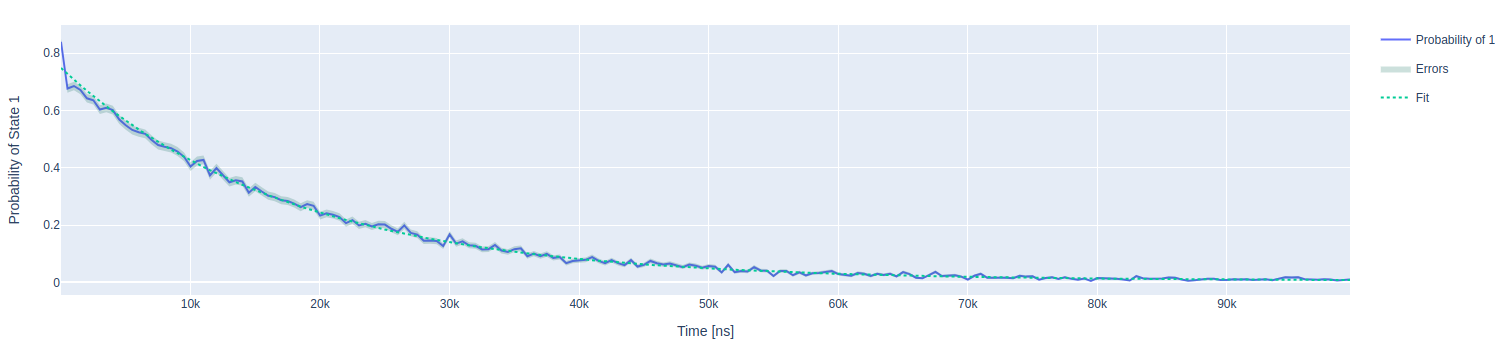
\includegraphics[width=\textwidth]{figures/png/t1.png}
    \caption{Output of the $T1$ measurement on qubit B2.}
    \label{fig:t1}
\end{figure}

After measuring $T_1$ it is necessary to measure also the dephasing time of the qubit, $T_2$; to do this in \Qibocal, it is possible to perform a T2 experiment.
The acquisition sequence of the experiment is the same as the Ramsey experiment described in Section \ref{subsec:Ramsey}: a pair of $\pi/2$-pulses is applied with a variable delay $\tau$ in between, during which the qubit freely evolves under a slightly detuned drive.
As a result, the measured excited state population exhibits oscillations in time, caused by the accumulation of phase due to the detuning. 
These oscillations are enveloped by an exponential decay that reflects the qubit's loss of phase coherence over time.  

In the T2 experiment the same pulse sequence is used with the caveat that the drive pulse is not detuned, the protocol assumes that any error on the drive frequency has already been corrected through a Ramsey experiment.
For this reason, the curve that describes the excited state population is expected to follow a simple exponential decay:
\begin{equation}
    p_e(t) = A + Be^{-\frac{t}{T_2}},
\end{equation}
where $A$ and $B$ are two fitting parameters.

\begin{figure}[h!]
    \centering
    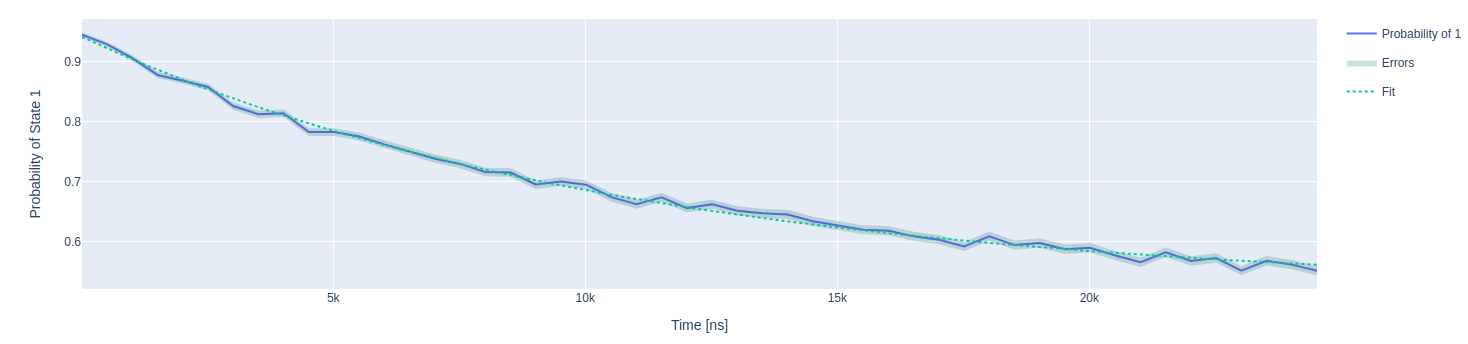
\includegraphics[width=\textwidth]{figures/png/t2.png}
    \caption{Output of the $T2$ measurement on qubit B2.}
    \label{fig:t2}
\end{figure}

\subsection{Standard Randomized Benchmarking}\label{sec:RB_calibration}
The standard randomized benchmarking experiment will be described in more detail in the following chapter (see Section \ref{sec:RBsection}).
For now, it is enough to say that in this routine, sequences of randomly selected Clifford gates are applied to the qubit, followed by an inverting gate that ideally returns the system to its initial state. 
By measuring the survival probability as a function of sequence length and fitting the decay curve, an estimate of the average gate fidelity is obtained.
An example of the output expected from the randomized benchmarking protocol is shown in Figure \ref{fig:rb}.

\begin{figure}[h!]
    \centering
    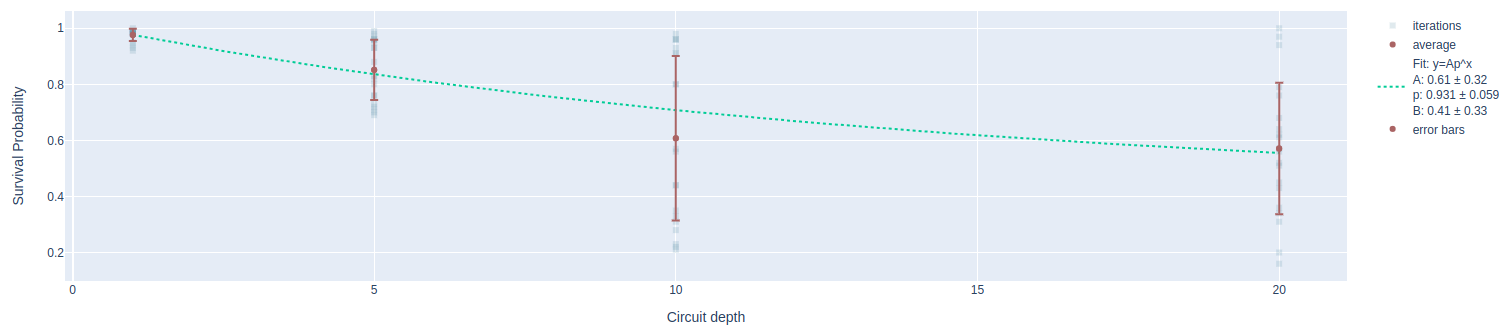
\includegraphics[width=\textwidth]{figures/png/rb.png}
    \caption{Output of the standard randomized benchmarking routine on qubit B2.}
    \label{fig:rb}
\end{figure}


\subsection{DRAG experiment}\label{sec:DRAG}
\subsubsection{DRAG pulse shape}
As mentioned in section \ref{sec:qubit_control}, the study of optimal pulse shapes (especially for drive and control pulses) is an active area of research. 
The Derivative Reduction by Adiabatic Gate (DRAG) technique \cite{Motzoi_2009}\cite{Gambetta_2011} is a widely used method to mitigate leakage errors during high-fidelity single-qubit gate operations.
The DRAG is the analytical solution to force the interaction Hamiltonian of the system \ref{eq:interaction_hamiltonian} to be restricted to the computational space.

The DRAG scheme implements a single-qubit rotation by applying a shaped pulse with an envelope $\Omega(t)$ on one quadrature (typically along $\hat{\sigma_x}$) and a secondary pulse with an envelope proportional to the time derivative $\dot{\Omega}(t)$ on the orthogonal quadrature (typically $\hat{\sigma_y}$).
For instance, a rotation about the $x$-axis is generated by the time-dependent Hamiltonian\cite{manenti_quantum_2023}:
\begin{equation}\label{eq:DRAG_hamiiltonian}
    \hat{H}_d(t) = \hbar \, \Omega_x(t) \sin(\omega_d t) \, \hat{\sigma}_x + \hbar \, \Omega_y(t) \sin(\omega_d t + \pi) \, \hat{\sigma}_y,
\end{equation}
where the pulse shapes are defined as:
\begin{align}
    \Omega_x(t) &= \Omega_0 e^{-t^2 / (2\sigma^2)}, \\
    \Omega_y(t) &= \lambda/\eta \frac{d}{dt} \Omega_x(t),
\end{align}
where $\eta$ represents the qubit anharmonicity and $\lambda$ is a dimensionless scaling parameter.
The efficacy of the DRAG correction arises from its ability to suppress virtual transitions that occur due to the spectral overlap of the primary pulse with off-resonant transitions in the multilevel qubit structure.

Theory predicts that setting $\lambda=1$ minimizes the leakage to higher excited stats, while $\lambda=0.5$ is optimal for correcting phase distortions induced during the gates \cite{Motzoi_2009}, \cite{Gambetta_2011}, \cite{Motzoi2013}.
In experimental implementations, the optimal value of $\lambda$ may deviate from theoretical predictions due to pulse distortions, the limited bandwidth of the control electronics, and interactions with the readout resonator \cite{PhysRevA.82.040305}.

\subsubsection{DRAG protocol}
A straightforward experiment implemented in \Qibocal to calibrate the $\lambda$ parameter involves performing two separate measurements using DRAG pulses in the pulse sequence.
In the first experiment, a sequence of DRAG pulses is applied in the order $Y_{\pi}$$X_{\frac{\pi}{2}}$ with both pulses parametrized by a given value of $\lambda$. 
For the second measurement, the procedure is the same but the pulse order is reversed $X_{\pi}$$Y_{\frac{\pi}{2}}$.
These specific sequences are chosen because they ideally result in the same final quantum state—any discrepancy between the two indicates phase misalignment, in particular, these sequences exhibit opposite signs of phase errors, as explained in \cite{reed2013entanglementquantumerrorcorrection}. 

The post-processing consists of measuring the probability of the qubit being in the state $\ket{1}$ for each value of $\lambda$. 
A linear fit is performed for both pulse sequences, and the correct $\lambda$ is the value where the two lines cross. 
This intersection corresponds to the $\lambda$ value that minimizes phase errors and ensures the qubit operates with minimal distortion.

An example of the expected output for the DRAG routine is shown in Figure \ref{fig:drag}
\begin{figure}[h!]
    \centering
    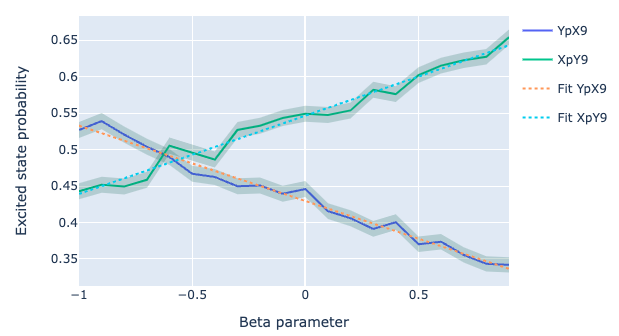
\includegraphics[width=0.5\textwidth]{figures/png/drag_simple.png}
    \caption{Expected output of the \tt{drag\_simple} routine. $\beta$ is the symbol used in \Qibocal for the $\lambda$ parameter.}
    \label{fig:drag}
\end{figure}

In \Qibocal is implemented also another routine that can be used to determine the correct value of the DRAG parameter $\beta$. This method employs a pulse sequence of the form
\begin{equation}
    [X_{\pi} - X_{-\pi}]^N,
\end{equation}
where the repeated application of positive and negative $\pi$-rotations amplifies coherent errors arising from imperfect pulse shaping. 
This approach is particularly sensitive to distortions introduced by an incorrectly tuned quadrature derivative component, which the DRAG technique is specifically designed to compensate for. 
By varying $\beta$, which scales the amplitude of the derivative pulse on the quadrature channel, one observes oscillations in the qubit's return probability to the ground state $\ket{0}$, caused by constructive and destructive interference of the accumulated errors.
The measured ground state population is recorded as a function of $\beta$ and fit to a cosine curve. 
The optimal value of $\beta$ corresponds to the point where this oscillation is maximized—indicating minimal leakage and optimal cancellation of phase errors. 
This approach to the calibration of the $\beta$ parameter was first introduced in \cite{DRAG2}. 
A possible output of the routine is shown in Figure \ref{fig:drag_tuning}.

\begin{figure}[h!]
    \centering
    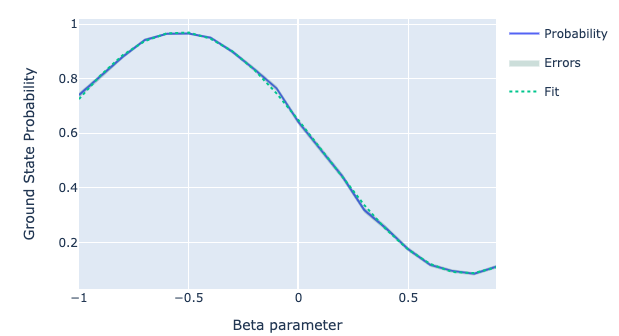
\includegraphics[width=0.5\textwidth]{figures/png/drag_tuning.png}
    \caption{Expected output of the \tt{drag\_tuning} routine.}
    \label{fig:drag_tuning}
\end{figure}

\section{Calibration results}

In Table \ref{tab:cal_results}, are summarized the results obtained for the calibration of line D of the \tt{qw11q} chip. 
The readout and assignment fidelities were obtained by performing a classification exèperiment on each qubit with 5000 shots, while $T1$ and $T2$ measurements were carried out using the respective protocols, each with $2048$ shots.\\
The standard randomized benchmarking was performed at four different circuit depths: $n=1,5,10,20$; for each depth the circuit was repeated $20$ times with $100$ shots per repetition. 
The number of shots in the randomized benchmarking experiment was deliberately limited, as this routine is inherently very time-consuming.

\begin{table}[h]
    \centering
    \begin{tabular}{lccccc}
    \toprule
    \textbf{Qubit} & \multicolumn{1}{c}{\textbf{Readout}} & \multicolumn{1}{c}{\textbf{Assignment}} & \textbf{T1 [$\mu$s]} & \textbf{T2 [$\mu$s]} & \textbf{Gate infidelity ($\cdot 10^{-3}$)} \\
    \textbf{} & \textbf{Fidelity} & \textbf{Fidelity} & & & \\
    \midrule
    \textbf{D1} & $0.876$ & $0.938$ & $26.4 \pm 0.4$ & $13.0 \pm 2.0$ & $27.0 \pm 21.0$ \\
    \textbf{D2} & $0.945$ & $0.973$ & $14.9 \pm 0.1$ & $18.0 \pm 10.0$ & $20.5 \pm 6.2$ \\
    \textbf{D3} & $0.905$ & $0.952$ & $23.6 \pm 0.3$ & $28.0 \pm 12.0$ & $7.0 \pm 18$ \\
    \textbf{D4} & $0.929$ & $0.964$ & $20.6 \pm 0.2$ & $38.0 \pm 5.2$ & $4.4 \pm 4.8$ \\
    \textbf{B2} & $0.902$ & $0.951$ & $17.5 \pm 0.2$ & $27.5 \pm 5.2$ & $18.0 \pm 16$ \\
    \bottomrule
    \end{tabular}
    \caption{Single qubit gates calibration results. D line was the first one I tried to calibrate.\\
    For completeness in the table, I report also the values for B2 which were calibrated lately for the purpose of showing calibration results in this chapter.}
    \label{tab:cal_results}
\end{table}

The values of the assignment fidelity and readout fidelity are overall satisfactory, indicating reliable state discrimination during measurement. 
Similarly, the relaxation time $T_1$ of the qubit shows acceptable values.

On the other hand, the coherence time $T_2$ is generally low, especially when considering that its theoretical upper bound is $2T_1$. 
This indicates the presence of significant pure dephasing mechanisms, which are limiting the coherence independently of energy relaxation processes. 
A reduced $T_2$ can have important consequences for subsequent experiments, particularly impacting the performance of randomized benchmarking protocols. 
Specifically, a short coherence time may degrade the fidelity of gate operations, leading to an overestimation of the average error per gate.

Undoubtedly, individuals with greater experience in the calibration of superconducting qubits are able to achieve significantly better figures of merit than those reported in table \ref{tab:cal_results}.
For comparison, the qubits on the chip used in this work are designed to achieve coherence times in the range of $T_1 = 29 - 39 \mu$s and $T_2 = 58 - 78 \mu$s, which are consistent with typical targets for high-performance superconducting qubits. 
In terms of fidelity, state-of-the-art calibration techniques currently achieve readout fidelities between $95\%$ and $99.5\%$ \cite{krantz_quantum_2019}, and single-qubit gate fidelities in the range of $99.5\%$ to $99.99\%$.
The satisfactory, yet overall limited, results obtained from this initial calibration can be partially attributed to a non-optimal calibration procedure and partially to limitations of the experimental setup, which could be further investigated.